% !TeX program = xelatex 

\PassOptionsToPackage{prologue, dvipsnames}{xcolor}
\documentclass[AutoFakeBold,AutoFakeSlant]{beamer}
\usetheme{metropolis}           % Use metropolis theme
\setbeamercovered{transparent}
\usepackage{listings}
\usepackage{ThinctPPT}
\usepackage[font=normalsize,labelfont=sf,textfont=sf]{subcaption} % Use only subcaption, not subfig
 
% 支持中文的设置
\usepackage{xeCJK}
\usepackage{fontspec}
\setCJKmainfont[ItalicFont=思源宋体,BoldFont=SourceHanSerifSC-Bold]{Source Han Serif SC}
\newcommand{\KaiTi}{\CJKfontspec{楷体}}%用命令\fzkaiti调用方正楷体简体

% other packages
\usepackage{latexsym,amsmath,xcolor,multicol,booktabs,calligra}
\usepackage{graphicx,pstricks,listings,stackengine}
\usepackage{wrapfig}

\title{\textbf{2023}\\年终总结}
\date{\today}
\author{
\includegraphics[width=0.26\linewidth]{logo}\\软件部-王升平}
\begin{document}
	\maketitle
	
	\section{过去一年的数据}
	\subsection{BUG数据}
	\begin{frame}[fragile]
		\LogoFrametitle{2023年度发现的BUG统计图表}
		\begin{figure*}
			\centering % 将整个 figure* 居中
			\begin{subfigure}{\linewidth}
				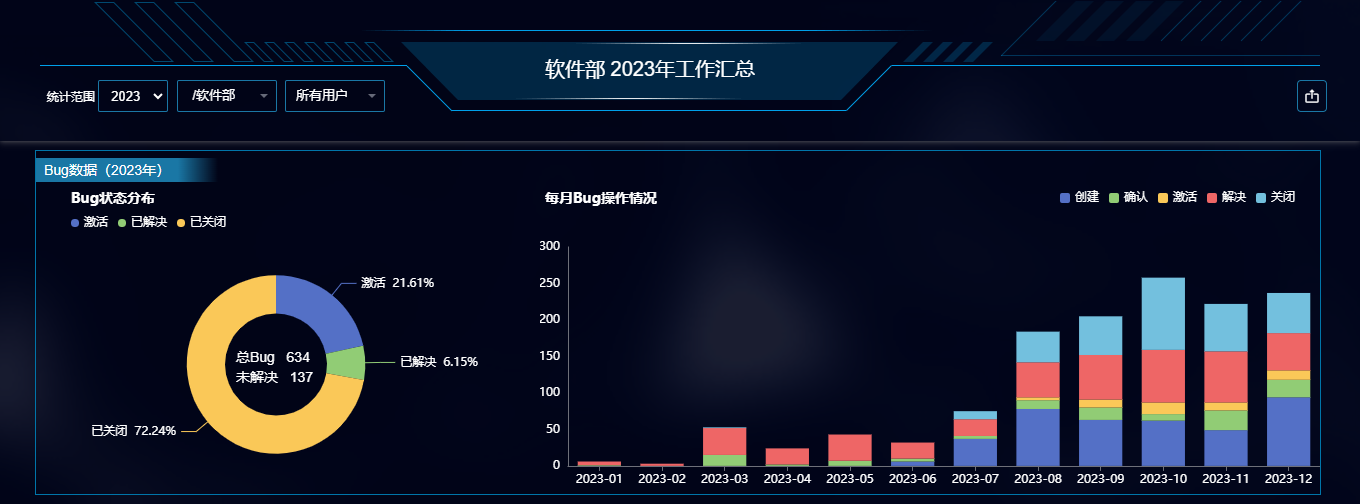
\includegraphics[width=\linewidth]{bug}
			\end{subfigure}
		\end{figure*} 
	\end{frame}
	
	\subsection{测试用例数据}
	\begin{frame}[fragile]
		\LogoFrametitle{EBX 代替当前的函数栈底}
	\end{frame}
	
	\subsection{开发任务数据}
	\begin{frame}[fragile]
		\LogoFrametitle{EBX 代替当前的函数栈底}
	\end{frame}
	
	
\end{document}
